\documentclass[a4paper, 11pt]{beamer}

\usepackage[T1]{fontenc}
\usepackage[polish]{babel}
\usepackage[utf8]{inputenc}
\usepackage{graphicx}
\usepackage{listings}
\usepackage{minted}
\usepackage{multicol}
\usepackage{graphicx}

\definecolor{bg}{rgb}{0.95,0.95,0.95}
\definecolor{bgr}{rgb}{0.95,0.60,0.60}

\usetheme{boxes} 

\begin{document}


\begin{frame}
\begin{centering}
\huge $\textit{IS-A}$ and $\textit{HAS-A}$ Relationship
\end{centering}
\end{frame}



\begin{frame}{$\textit{IS-A}$ relationship}
\begin{itemize}
\item expressed with class inheritance or interface implementation
\item 'this thing is a type of that thing'
\item cat is a animal
\item String is a Object
\item Triangle is a Shape
\end{itemize}
\end{frame}



\begin{frame}{$\textit{IS-A}$ Relationship}
\centering
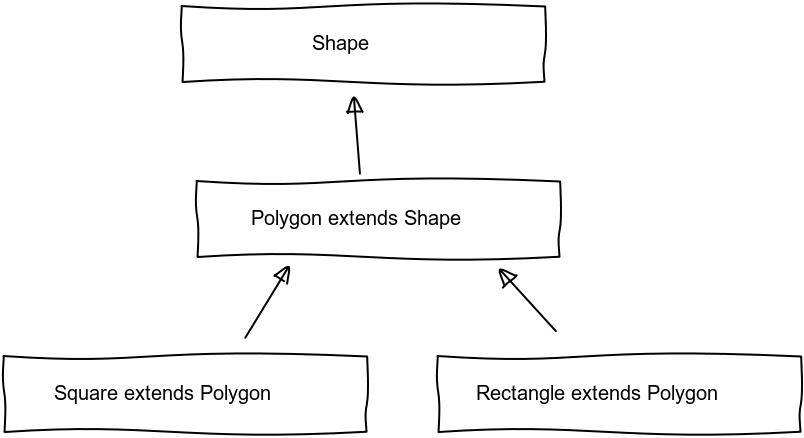
\includegraphics[scale=0.3]{img/isa.png}
\end{frame} 

\begin{frame}{$\textit{HAS-A}$ Relationship}
\begin{itemize}
\item is base on usage, rather than inheritance
\item instance of a class Triangle has reference to instance of a class Point
\end{itemize}
\end{frame}

\begin{frame}{$\textit{HAS-A}$ Relationship}
\centering
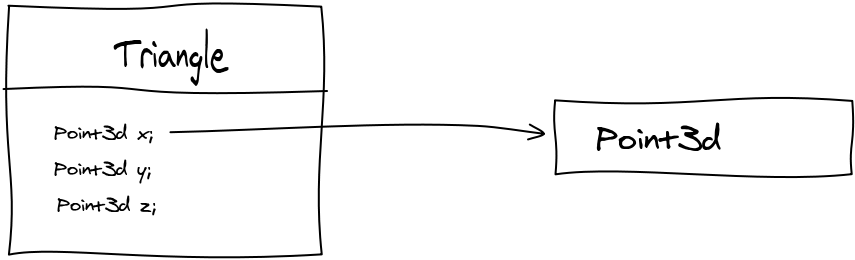
\includegraphics[scale=0.3]{img/hasa.png}
\end{frame}

\begin{frame}{Polymorphism}
Polymorphism is the ability of an object to take on many forms
\end{frame}

\begin{frame} { Type of polymorphism }

\begin{itemize}
\item $\textit{ad-hoc}$ - methods overloading vs overriding
\item parametric
\item dynamic method binding
\end{itemize}

\end{frame}

\begin{frame}{Dynamic method binding}

The ability of a program to resolve references to subclass methods at runtime. For example assume that three subclasses (Square, Rectangle,Triangle) have been created based on the Shape abstract class, each having their own calculateArea() method. Although each method reference is to an Shape (but no shape objects exist), the program is will resolve the correct method reference at runtime.

\end{frame}

\begin{frame}{$\textit{Overridden methods}$}

Methods that are redefined within an inherited or subclass. They have the same signature and the subclass definition is used.

\end{frame}

\begin{frame}{example}
\inputminted[bgcolor=bg, fontsize=\tiny]{java}{./src/overriding/Polygon.java}
\end{frame}


\begin{frame}{test}

\begin{columns}
    \begin{column}{.3\linewidth}
      \inputminted[bgcolor=bg, fontsize=\tiny]{java}{./src/overriding/Polygon.java}        
    \end{column}
%    \newcolumn
\vline
%%%%%\columnbreak
    \begin{column}{.5\linewidth}
       \inputminted[bgcolor=bg, fontsize=\tiny]{java}{./src/overriding/PolygonTest.java}
   
    \end{column}
  \end{columns}
\end{frame}

\begin{frame}{test - FAIL}

\begin{columns}
    \begin{column}{.3\linewidth}
      \inputminted[bgcolor=bg, fontsize=\tiny]{java}{./src/overriding/Polygon.java}        
    \end{column}
%    \newcolumn
\vline
%%%%%\columnbreak
    \begin{column}{.5\linewidth}
       \inputminted[bgcolor=bg, fontsize=\tiny]{java}{./src/overriding/PolygonTestFail.java}
   
    \end{column}
  \end{columns}
\end{frame}


\begin{frame}{test}

\begin{columns}
    \begin{column}{.3\linewidth}
      \inputminted[bgcolor=bg, fontsize=\tiny]{java}{./src/overriding/Polygon.java}        
    \end{column}
%    \newcolumn
\vline
%%%%%\columnbreak
    \begin{column}{.5\linewidth}
       \inputminted[bgcolor=bg, fontsize=\tiny]{java}{./src/overriding/PolygonTest2.java}
   
    \end{column}
  \end{columns}
\end{frame}

\begin{frame}{test}

\begin{columns}
    \begin{column}{.3\linewidth}
      \inputminted[bgcolor=bg, fontsize=\tiny]{java}{./src/overriding/Polygon.java}        
    \end{column}
%    \newcolumn
\vline
%%%%%\columnbreak
    \begin{column}{.5\linewidth}
       \inputminted[bgcolor=bg, fontsize=\tiny]{java}{./src/overriding/PolygonTest2Fail.java}
   
    \end{column}
  \end{columns}
\end{frame}


\begin{frame}{example}
\inputminted[bgcolor=bg, fontsize=\tiny]{java}{./src/overriding/Polygon2.java}
\end{frame}

\begin{frame}{test}

\begin{columns}
    \begin{column}{.3\linewidth}
      \inputminted[bgcolor=bg, fontsize=\tiny]{java}{./src/overriding/Polygon2.java}        
    \end{column}
%    \newcolumn
\vline
%%%%%\columnbreak
    \begin{column}{.5\linewidth}
       \inputminted[bgcolor=bg, fontsize=\tiny]{java}{./src/overriding/Polygon2Test.java}
   
    \end{column}
  \end{columns}
\end{frame}

\begin{frame}{test - result}

\begin{columns}
    \begin{column}{.3\linewidth}
      \inputminted[bgcolor=bg, fontsize=\tiny]{java}{./src/overriding/Polygon2.java}        
    \end{column}
%    \newcolumn
\vline
%%%%%\columnbreak
    \begin{column}{.5\linewidth}
       \inputminted[bgcolor=bg, fontsize=\tiny]{java}{./src/overriding/Polygon2TestFail.java}
   
    \end{column}
  \end{columns}
\end{frame}


%%%%%%%%%%%%%%%%%%%%%%%%%%%%%%%%%%%%%%%%



\begin{frame}{example}
\inputminted[bgcolor=bg, fontsize=\tiny]{java}{./src/overriding/Polygon3.java}
\end{frame}

\begin{frame}{test}

\begin{columns}
    \begin{column}{.3\linewidth}
      \inputminted[bgcolor=bg, fontsize=\tiny]{java}{./src/overriding/Polygon3.java}        
    \end{column}
%    \newcolumn
\vline
%%%%%\columnbreak
    \begin{column}{.5\linewidth}
       \inputminted[bgcolor=bg, fontsize=\tiny]{java}{./src/overriding/Polygon3Test.java}
   
    \end{column}
  \end{columns}
\end{frame}

\begin{frame}{test - result}

\begin{columns}
    \begin{column}{.3\linewidth}
      \inputminted[bgcolor=bg, fontsize=\tiny]{java}{./src/overriding/Polygon3.java}        
    \end{column}
%    \newcolumn
\vline
%%%%%\columnbreak
    \begin{column}{.5\linewidth}
       \inputminted[bgcolor=bg, fontsize=\tiny]{java}{./src/overriding/Polygon3TestFail.java}
   
    \end{column}
  \end{columns}
\end{frame}


\begin{frame}{Rules}
\begin{itemize}
\item the argument list must exactly match that of the overridden method. If they
don't match, you can end up with an overloaded method you didn't intend.
\item  the return type must be the same as, or a subtype of, the return type declared
in the original overridden method in the superclass. 
\item the access level can't be more restrictive than the overridden method's.
\item the access level CAN be less restrictive than that of the overridden method.
\item you cannot override a method marked final.
\item you cannot override a method marked static.
\end{itemize}
\end{frame}



%%%%%%%%%%%%%%%%%%%%%%%%%%%%%%%%%%%%%%%%



\begin{frame}{example}
\inputminted[bgcolor=bg, fontsize=\tiny]{java}{./src/overriding/Polygon4.java}
\end{frame}

\begin{frame}{test}

\begin{columns}
    \begin{column}{.3\linewidth}
      \inputminted[bgcolor=bg, fontsize=\tiny]{java}{./src/overriding/Polygon4.java}        
    \end{column}
%    \newcolumn
\vline
%%%%%\columnbreak
    \begin{column}{.5\linewidth}
       \inputminted[bgcolor=bg, fontsize=\tiny]{java}{./src/overriding/Polygon4Test.java}
   
    \end{column}
  \end{columns}
\end{frame}

\begin{frame}{test - result}

\begin{columns}
    \begin{column}{.3\linewidth}
      \inputminted[bgcolor=bg, fontsize=\tiny]{java}{./src/overriding/Polygon4.java}        
    \end{column}
%    \newcolumn
\vline
%%%%%\columnbreak
    \begin{column}{.5\linewidth}
       \inputminted[bgcolor=bg, fontsize=\tiny]{java}{./src/overriding/Polygon4TestFail.java}
   
    \end{column}
  \end{columns}
\end{frame}

\begin{frame}{Overloaded method}

Methods with the same name signature but either a different number of parameters or different types in the parameter list.

\end{frame}


\begin{frame}{Rules}

\begin{itemize}
\item overloaded methods MUST change the argument list.
\item overloaded methods CAN change the return type.
\item overloaded methods CAN change the access modifier.
\item overloaded methods CAN declare new or broader checked exceptions.

\end{itemize}


\end{frame}

\begin{frame}{example}
\inputminted[bgcolor=bg, fontsize=\tiny]{java}{./src/overloading/Polygon3.java}
\end{frame}

\begin{frame}
Polymorphic method invocations apply only to instance methods. You can
always refer to an object with a more general reference variable type (a su-
perclass or interface), but at runtime, the ONLY things that are dynamically
selected based on the actual object (rather than the reference type) are instance
methods. Not static methods. Not variables. Only overridden instance meth-
ods are dynamically invoked based on the real object's type.


\end{frame}

\begin{frame}{Comparison operators}

Two operators
\begin{itemize}
\item $\textit{==}$
\item $\textit{.equals()}$
\end{itemize}
\end{frame}

\begin{frame}
\inputminted[bgcolor=bg, fontsize=\tiny]{java}{./src/equal/Equal.java}
\end{frame}

%%%%%%%%%%%%%%%%%%%%%%%%%%%%%%%%%%%%%%%%%%%%%%%%%

\begin{frame}{test}

\begin{columns}
    \begin{column}{.3\linewidth}
      \inputminted[bgcolor=bg, fontsize=\tiny]{java}{./src/equal/Equal.java}        
    \end{column}
%    \newcolumn
\vline
%%%%%\columnbreak
    \begin{column}{.5\linewidth}
       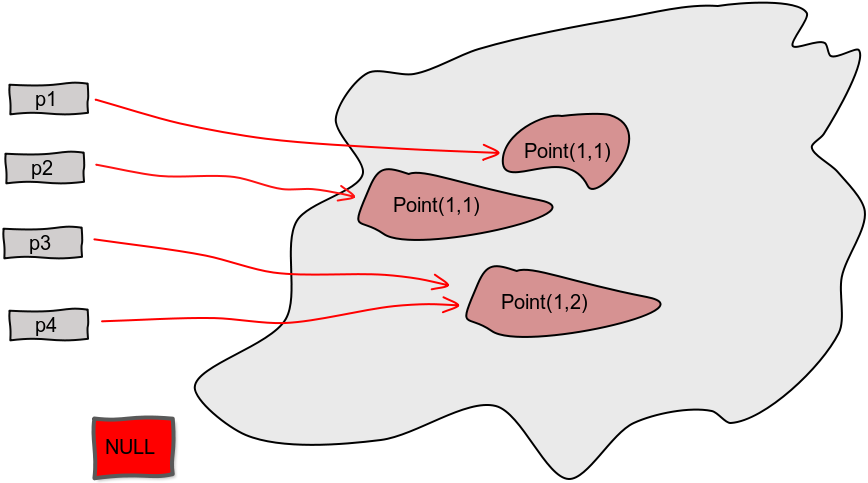
\includegraphics[scale=0.2]{img/equal.png}
   
    \end{column}
  \end{columns}
\end{frame}

%%%%%%%%%%%%%%%%%%%%%%%%%%%%%%%%%%%%%%%%%%%%%%%%%

\begin{frame}{test}

\begin{columns}
    \begin{column}{.3\linewidth}
      \inputminted[bgcolor=bg, fontsize=\tiny]{java}{./src/equal/EqualFalse.java}        
    \end{column}
%    \newcolumn
\vline
%%%%%\columnbreak
    \begin{column}{.5\linewidth}
       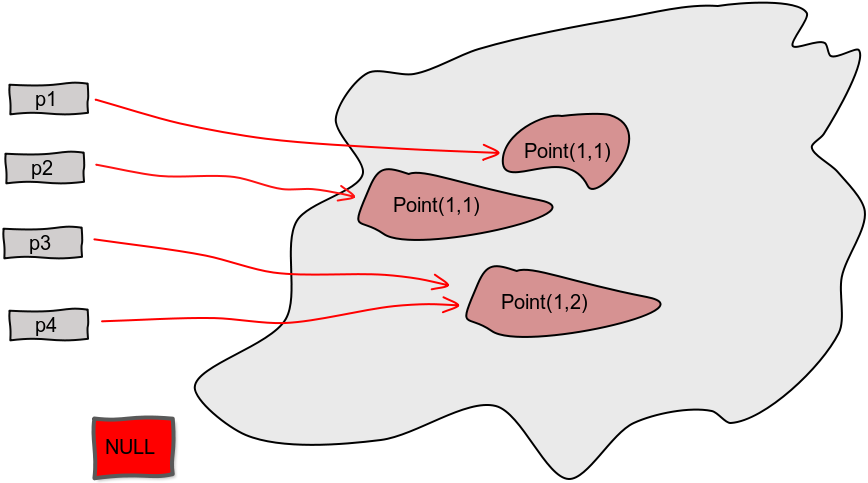
\includegraphics[scale=0.2]{img/equal.png}
   
    \end{column}
  \end{columns}
\end{frame}



%%%%%%%%%%%%%%%%%%%%%%%%%%%%%%%%%%%%%%%%%%%%%%%%%

\begin{frame}{compare different object}

\begin{columns}
    \begin{column}{.3\linewidth}
      \inputminted[bgcolor=bg, fontsize=\tiny]{java}{./src/equal/EqualFalseResult.java}        
    \end{column}
%    \newcolumn
\vline
%%%%%\columnbreak
    \begin{column}{.5\linewidth}
       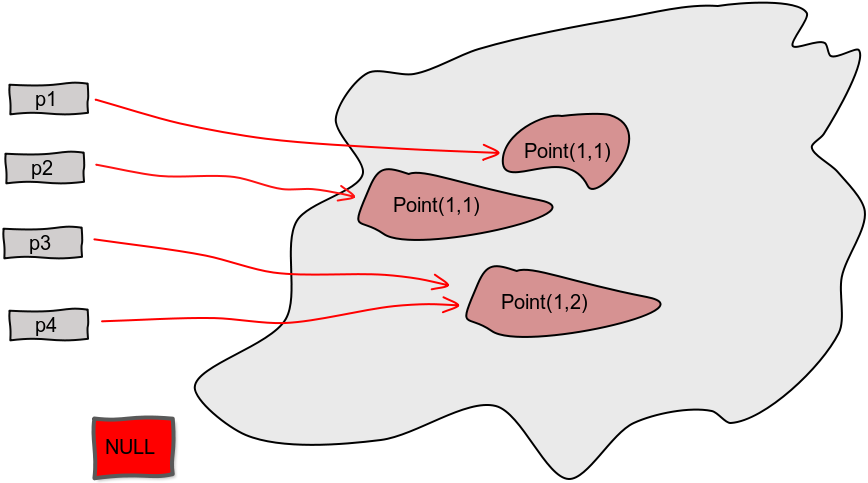
\includegraphics[scale=0.2]{img/equal.png}
   
    \end{column}
  \end{columns}
\end{frame}


%%%%%%%%%%%%%%%%%%%%%%%%%%%%%%%%%%%%%%%%%%%%%%%%%

\begin{frame}{compare references object}

\begin{columns}
    \begin{column}{.3\linewidth}
      \inputminted[bgcolor=bg, fontsize=\tiny]{java}{./src/equal/EqualRef.java}        
    \end{column}
%    \newcolumn
\vline
%%%%%\columnbreak
    \begin{column}{.5\linewidth}
       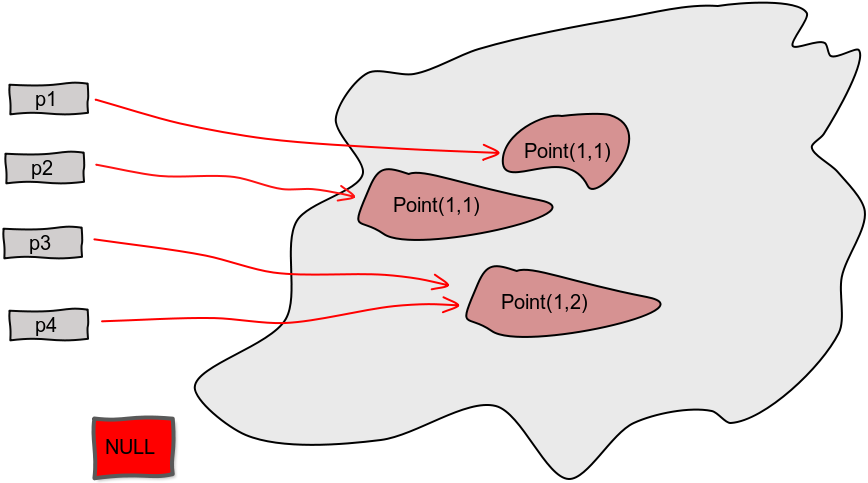
\includegraphics[scale=0.2]{img/equal.png}
   
    \end{column}
  \end{columns}
\end{frame}
%%%%%%%%%%%%%%%%%%%%%%%%%%%%%%%%%%%%%%%%%%%%%%%%%

\begin{frame}{compare references object}

\begin{columns}
    \begin{column}{.3\linewidth}
      \inputminted[bgcolor=bg, fontsize=\tiny]{java}{./src/equal/EqualRef2.java}        
    \end{column}
%    \newcolumn
\vline
%%%%%\columnbreak
    \begin{column}{.5\linewidth}
       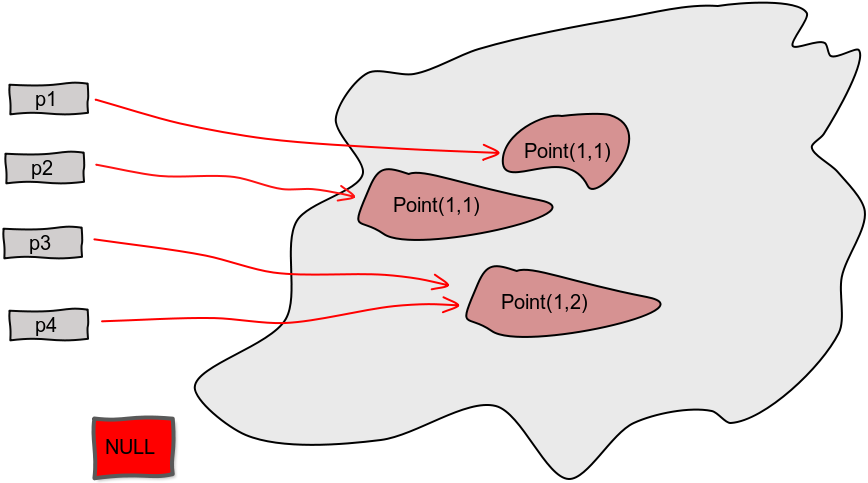
\includegraphics[scale=0.2]{img/equal.png}
   
    \end{column}
  \end{columns}
\end{frame}


%%%%%%%%%%%%%%%%%%%%%%%%%%%%%%%%%%%%%%%%%%%%%%%%%

\begin{frame}{compare references object}

\begin{columns}
    \begin{column}{.3\linewidth}
      \inputminted[bgcolor=bg, fontsize=\tiny]{java}{./src/equal/EqualRef2Result.java}        
    \end{column}
%    \newcolumn
\vline
%%%%%\columnbreak
    \begin{column}{.5\linewidth}
       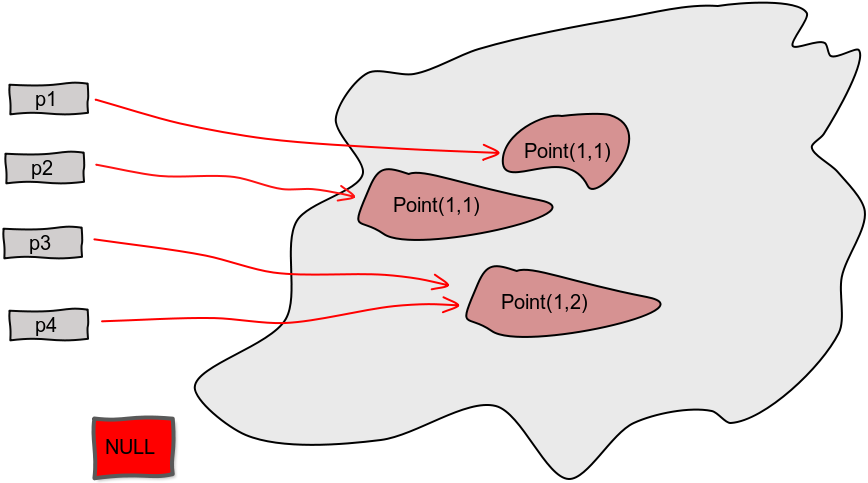
\includegraphics[scale=0.2]{img/equal.png}
   
    \end{column}
  \end{columns}
\end{frame}


\end{document}
